\documentclass[12pt,a4paper]{scrartcl}

\usepackage{hyperref}
\usepackage{url}
\usepackage{graphicx}
\usepackage{xcolor}
\usepackage{textcomp}
\usepackage{subfig}
\usepackage{amsmath}

\definecolor{steelblue}{rgb}{0.36, 0.54, 0.66}

\newcommand{\git}[0]{\href{https://git.hhu.de/machne/pbr_hackathon_201503}{PBR git}}
\newcommand{\ordered}[0]{\textcolor{steelblue}{\textbf{ordered}}}
\newcommand{\obtain}[0]{\textcolor{orange}{\textbf{obtain}}}
\newcommand{\avail}[0]{\textcolor{green}{\textbf{available}}}
\newcommand{\build}[0]{\textcolor{red}{\textbf{build}}}
\newcommand{\code}[0]{\textcolor{blue}{\textbf{code}}}
\newcommand{\hack}[0]{Hack`a'thing}
\newcommand{\gasometer}[0]{\texttt{Gas`o'meter}}
\newcommand{\ph}[0]{h{\small$^{-1}$}}
\newcommand{\ox}[0]{O$_2$}
\newcommand{\cox}[0]{CO$_2$}

\parskip 0.3 cm
\parindent 0 cm

\title{1$^{st}$ QTB PBR \hack{}}
\subtitle{Soldering for and by beginners.}
\date{March 2--4, 2016}

\begin{document}
\maketitle
%\scriptsize
\tableofcontents
%\normalsize
\newpage


\section{Program}

\subsection{March 2 $<$12:00 : Building Bioreactors}

Talks, 30-60 min:
\begin{itemize}
\item Rob's DIY Reactor - The Beginnings: \texttt{NinjaPBR} -
  Arduino-controlled mini PBR
\item Dougie's DIY Reactor - 20 yrs Later
\item Avantes - Spectrometry: Spectrometry applications, incl. NIR for
  metabolite measurements and OD; software interface to Avantes
  spectrometers
\item CellDeg - Optimizing Photosynthetic Growth: Introduction to
  CellDeg's 2.5 k Euro algal growth setup (30 g/L cyano
  biomass in three days)
\end{itemize}


\subsection{March 2 $>$13:00 : \hack{} I}

\begin{itemize}
\item Introduction to the \gasometer{}: connecting sensors with Arduino,
  making an autonomous measurement device via Sainsmart's Touch Screen
\item Introduction to Rob's reactor: complete setup for photosynthetic growth
\item Introduction to 3D printing with QTB's \texttt{ultimaker$^2$}
\item Self-organizing into teams: lab hardware (tubing etc.), control hardware
(soldering etc.), software and/or by by projects (\ref{gas}--\ref{micro}) 
\end{itemize}

\subsection{March 3 : \hack{} II}

%Perhaps in teams, either by projects (\ref{gas}--\ref{micro}) or in
%software vs. hardware (soldering/tubing) vs. biolab (cell cultures),
%or -- most likely -- in dynamic self-organisation, working parallel on
%all projects.

\begin{itemize}
\item Hardware I: soldering, tubing \& 3D printing
\item Software I: probe/sensor/pump $\Leftrightarrow$ arduino/raspi interfaces
\item Visit HHU's fine mechanics and glas blower work-shops, place
  orders
\end{itemize}

\subsection{March 4 : \hack{} III}

\begin{itemize}
\item Hardware II: Integrate projects \ref{gas},\ref{spec}\&\ref{cult}
  into a simple DIY reactor and/or with PSI FMT150 or Multicultivator
%\item 
%\end{itemize}
%\subsection{Day 3 $>$13:00 : Consolidating}
%\begin{itemize}
\item Software II: arduino/raspi $\Leftrightarrow$  master/server interface; data formats and interfaces
\item Brain storming: relation of data and models and beer
%\item Beer: relation of data and models and beer
\end{itemize}

\subsection*{Resources - Materials, Designs and Ideas}

Please see the
\href{https://wiki.hhu.de/display/QTBP/1st+QTB+PBR+Hack\%60a'thing}{Hack`a'thing
  Wiki} for link lists of DIY bioreactors, DIY lab ware, 3D printer
designs, general DIY websites, and electronics suppy shops.

This program and all code is at the \href{https://git.hhu.de/machne/pbr_hackathon_201503/tree/master}{HHU git project}.

\begin{figure}[ht]
  \begin{minipage}{.49\textwidth}
    \subfloat[Dougie's Reactor]{
      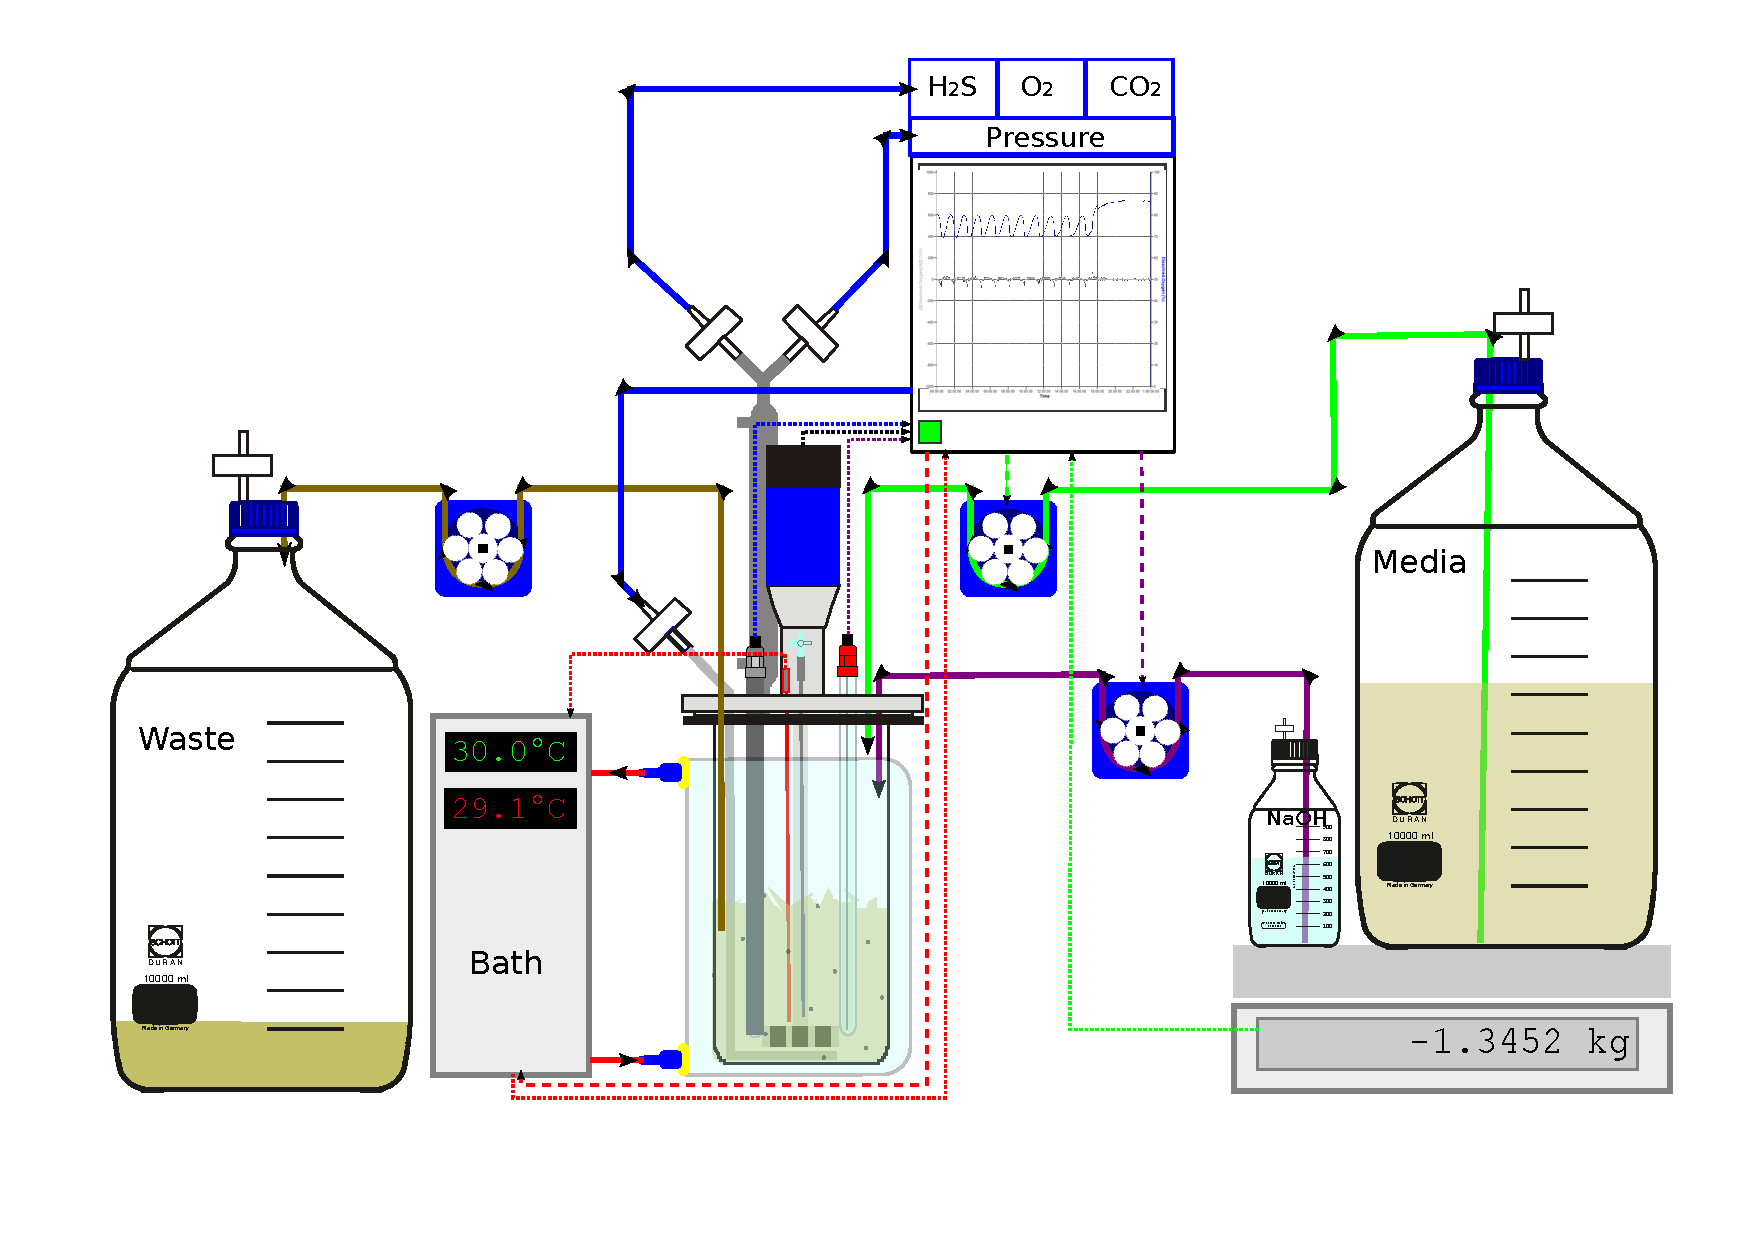
\includegraphics[width=\textwidth]{figures/fermentor_detailed.pdf}\\ 
    }
  \end{minipage}
  \begin{minipage}{.49\textwidth}
    \centering Monod: $\mu = \mu_{max} \frac{S}{S+K_S}$\\
    \subfloat[Snoep \textit{et al.} 2009]{
      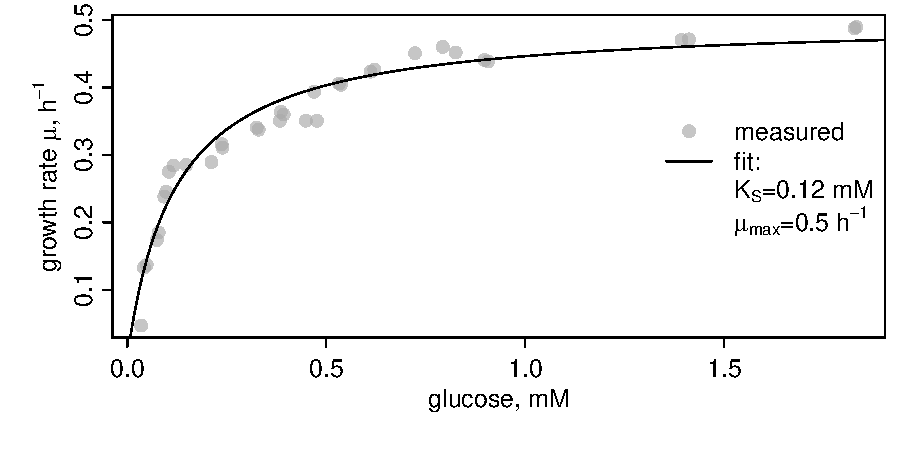
\includegraphics[width=\textwidth]{figures/snoep09_fig2.pdf}
    }
  \end{minipage}
\caption[]{Bioreactors}
\end{figure}

%\vspace{-10ex}

\begin{figure}
\begin{minipage}{.5\textwidth}
  \begin{equation*}
    \label{eqn:ancat}
    \begin{aligned}
      \frac{\text{d}X}{\text{d}t} &= (\mu_{ab} - \phi) X  \\
      \frac{\text{d}S}{\text{d}t} &= \phi (S_{in} - S)-(\mu_{ab} + \mu_{cd}) X\\  
      \frac{\text{d}atp}{\text{d}t} &= (n_{cd} \mu_{cd} - n_{ab} \mu_{ab} - \mu_{m})\frac{C_c}{V_c} - \mu_{ab} atp\\
      \frac{\text{d}G}{\text{d}t} &= k_La (G_{in}^* - G) - n_{g} \mu_{cd} X\\
      adp & = a_{tot} - atp
    \end{aligned}
  \end{equation*}
\end{minipage}
\begin{minipage}{.5\textwidth}
  \begin{equation*}
    \begin{aligned}
      \mu_{ab} &\equiv f(S,atp)\\
      \mu_{cd} &\equiv f(S,G,adp)\\
      \mu_m &\equiv f(S,ROS)
      n_{cd},\,n_{ab} &\equiv f(S) 
    \end{aligned}
  \end{equation*}
\end{minipage}
\caption{Growth in Continuous Culture: liquid and gas flux equations} 
\end{figure}

%\paragraph{DIY Bioreactors:}
%\begin{itemize}
%\item \href{http://www.yo-que.ch/nmrlab/mediawiki-1.15.1/index.php/Bioreactor}{Open source DIY bioreactor} and its \href{https://github.com/bioreactor}{code on github}
%\item \href{https://github.com/Bioreactor/Code-Bioreactor}{Github project for Arduino-controlled bioreactor}
%\item \href{http://onlinebioreactor.org/}{Onlinebioreactor: Arduino wiring schematics and source code for a temperature and pH measurements of a bioreactor}
%\item \href{http://www.instructables.com/id/An-Algae-Bioreactor-from-Recycled-Water-Bottles/}{An Algae Bioreactor from Recycled Water Bottles}
%\item \href{https://groups.google.com/forum/#!msg/diybio/j1oucFRuPUk/zz1Y_gE0PJkJ}{Google Group: DIY Bioreactor and Bioreactor controller}
%\item \href{http://jun.ucsd.edu/mother_machine.php}{The Jun lab's Mother Machine}
%\item \href{http://www.pellinglab.net/diy/diyco2incubator/}{Pelling lab's CO2 incubator for mammalian cell culture}
%\item \href{http://www.instructables.com/id/Biomonstaaar/}{Biomonstaaar: PBR instructable}, and \href{http://www.spacegambit.org/files/project_proposals/BioMONSTAAAR.pdf}{spacegambit project proposal}
%\item \href{http://www.openbioreacteurs.org/wiki/introduction/}{Openbioreacteurs: DIY algae reactors}
%\end{itemize}
%\paragraph{3D Printed Labware and Bioreactors:}
%\begin{itemize}
%\item \href{http://www.ncbi.nlm.nih.gov/pmc/articles/PMC4641590/}{Tsuda \textit{et al.} PLoS ONE 2015: 3D Printed 'Plug and Play' Millifluidic Devices}
%\item \href{http://onlinelibrary.wiley.com/doi/10.1002/elsc.201400093/abstract}{L\"ucking \textit{et al.} Eng. Life Sci. 2015: 3D printed labware, incl. ``well plate with different baffle geometries, shake flask cap with built-in luer connections, and filter holder for an in-house developed membrane reactor system''}; also see \href{http://jbioleng.biomedcentral.com/articles/10.1186/1754-1611-8-18}{paper by B\"uchs group on baffle geometries}
%\item \href{http://journals.plos.org/plosbiology/article?id=10.1371/journal.pbio.1002086}{Baden \textit{et al.} PLoS ONE 2015: Open Labware: 3-D Printing Your Own Lab Equipment}
%\end{itemize}
%
%\paragraph{Designs \& Instructions:}
%\begin{itemize}
%\item \href{http://playground.arduino.cc/}{Arduino Playground}: Wiki for Arduino-based Designs
%\item \href{http://www.instructables.com/}{Instructables}: Diverse DIY Designs
%\item \href{https://www.thingiverse.com/}{Thingiverse}: 3D Printer Designs
%\end{itemize}
%
%\paragraph{Shops:}
%\begin{itemize}
%\item \href{https://www.conrad.de/de/bauelemente-t04.html}{Conrad}: online and offline shop, DE
%\item \href{http://www.elecrow.com/}{Elecrow}: online shop, China
%\item \href{https://www.adafruit.com/}{Adafruit}: online shop, USA
%\item \href{https://www.fasttech.com/}{Fasttech}: online shop, China
%\end{itemize}

\newpage
\section{PBR \hack{} Awards}

\begin{itemize}
\item The ``most creative Arduino fry'' Award, inspiration at \href{https://www.youtube.com/watch?v=WmcMrKELkcs}{youtube: 5 ways to destroy}
\item The ``red soldering iron'' Award
\item The ``chip monkey'' Award
\end{itemize}

\newpage
\section{PBR \hack{} Projects}
\label{proj}

\subsection{Gas Flux: \gasometer{}}
\label{gas}
\paragraph{Project:} 
Extend existing setup (co2meter's
\href{http://www.co2meter.com/collections/co2-sensors/oxygen-sensors}{\ox{}}
and
\href{http://www.co2meter.com/collections/co2-sensors/products/cozir-5-100-co2-sensor}{\cox{}}
sensors with Sainsmart's
\href{http://www.sainsmart.com/featured-products/sainsmart-mega2560-board-3-5-tft-lcd-module-display-shield-kit-for-atmel-atmega-avr-16au-atmega8u2.html}{Arduino
  Mega+Touch screen}) by our brand new digital mass flow meter
\href{http://www.aalborg.com/index.php/main_page/product_overview/id_product_overview/63}{Aalborg
  XFM}; write calibration routines for all sensors; build water trap
and tubing to connect to the PSI or our DIY reactor and increase gas
transfer (smaller bubbles) and decrease overall gas flow so that we
can measure cellular activity. Perhaps add valve control to measure
multiple reactors in series.

\begin{enumerate}
\item \build{} water trap, tubing path from reactor, and casing for
  sensors and Arduino; \build{} improved gassing system (glas
  blowers!) to allow lower flow
\item \code{} sensor calibration routines via touch-screen (use PSI
  gas mixing system)
\item \build{} \& \code{} interface to Aalborg XFM digital mass flow
  meter: connect the Aalborg's RS 485 interface to Arduino hardware
  serial Tx3/Rx3, and Ground
\item \build{} \& \code{} valve control to measure several reactors;
  connect via Arduino software serial connections; perhaps attach to
  PSI Multicultivator
\end{enumerate}

\paragraph{Resources:}
\begin{itemize}
\item Sensor manuals in \texttt{code/manuals/offgas/} at the
  \git{}:\\
  \texttt{Manual-CM-0201-UV-Flux-Oxygen.pdf},
  \texttt{Manual-GSS-Sensors.pdf}, and\\
  \texttt{A\_XFM\_Manual\_TD0701M[...].pdf}
\item Code in  \texttt{code/offgas/arduino/} at the
  \git{}
\end{itemize}

\paragraph{Materials:}

\begin{itemize}
\item Existing setup: \avail{}
\item Aalborg XFM, with RS 485 interface: \avail{}
\item Valve system for gas tubing, controllable \textit{via} serial
  interface: \obtain{}
\end{itemize}

\begin{figure}[ht]
  \begin{minipage}{.49\textwidth}
    \subfloat[The Gas`o'meter: making of]{
      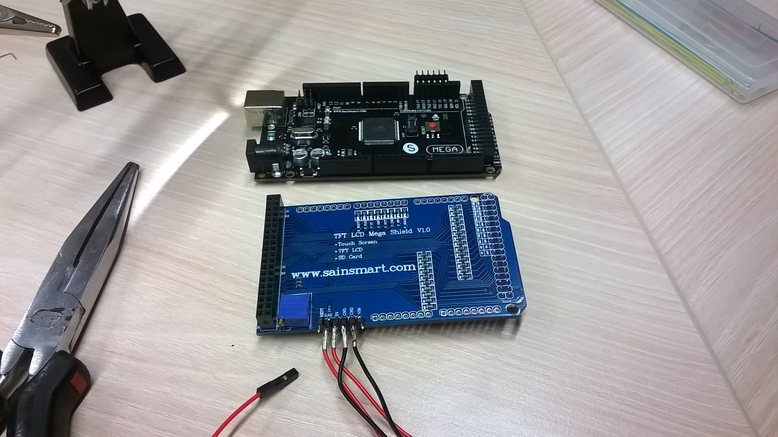
\includegraphics[width=\textwidth]{figures/offgas_makingof1.png}
    }
  \end{minipage}
  \begin{minipage}{.49\textwidth}
    \subfloat[The Gas`o'meter: making of]{
      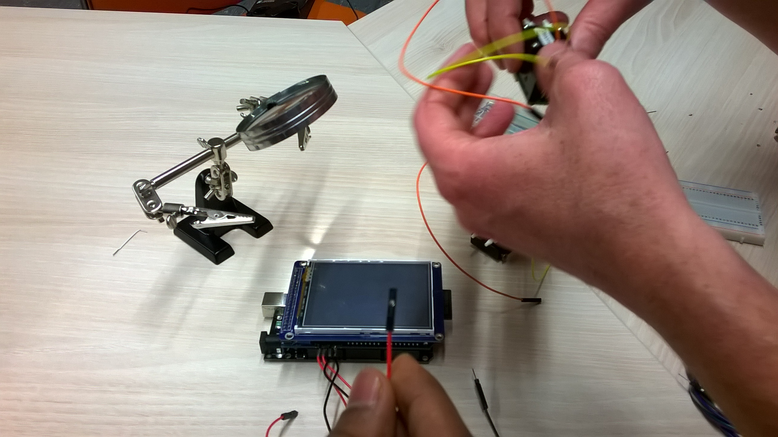
\includegraphics[width=\textwidth]{figures/offgas_makingof2.png}
    }
  \end{minipage}

  \begin{minipage}{.49\textwidth}
    \subfloat[The Gas`o'meter]{
      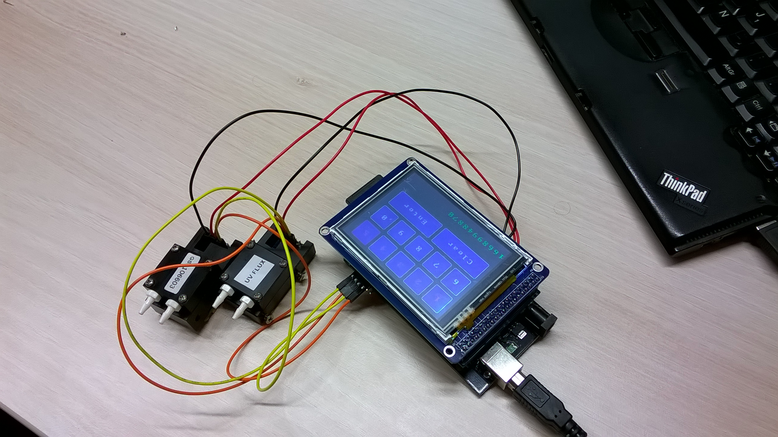
\includegraphics[width=\textwidth]{figures/offgas_makingof3.png}
    }
  \end{minipage}
  \begin{minipage}{.49\textwidth}
    \subfloat[Room 03.30, 2016-01-13]{
      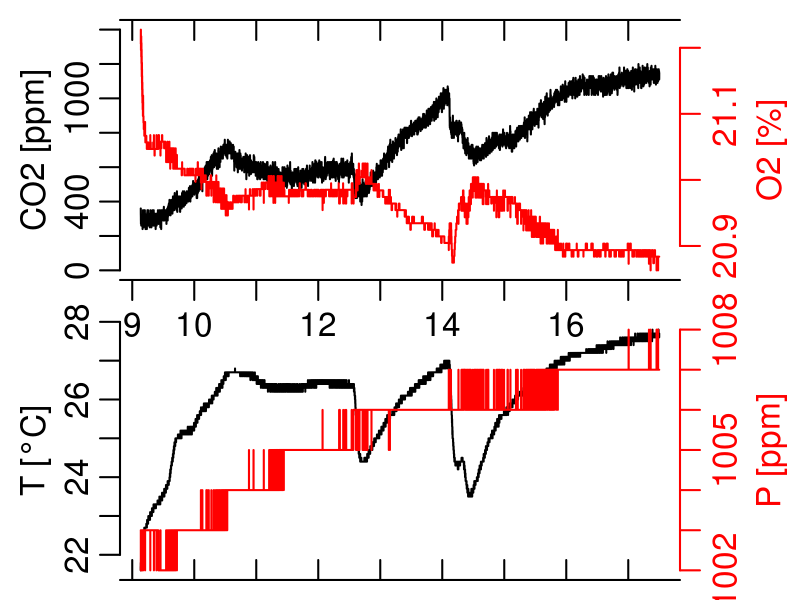
\includegraphics[width=\textwidth]{figures/20160113.png}
    }
  \end{minipage}
\caption[]{\textbf{Gas Measurement Module.}}
\end{figure}

\clearpage
\subsection{Light Flux: Spectrometer} 
\label{spec}
\paragraph{Project:} 
Simple spectrometric measuring tool based on
\href{http://www.avantes.com/products/spectrometers/compactline/item/723-avaspec-mini}{AvaSpec-Mini2048l-V25}

\begin{enumerate}
\item Basic: Connect to Rasperry Pi, using drivers provides by
  Avantes; \code{} simple interface with display and/or recording
  functions
\item Advanced: use LED for absorbance, reflectance, or fluorescence
  measurements; \build{} light paths and perhaps a reactor probe for
  online recording
\end{enumerate}


\paragraph{Resources:}
\begin{itemize}
\item
  \href{http://www.avantes.com/images/productsheets/AvaSpec_Mini5.pdf}{AvaSpec-Mini
    data sheet} in \texttt{code/manuals/light/} at the \git{}
\item \href{http://www.avantes.com/products/oem/item/220-oem-spectrometers-as5216-microprocessor-board}{The AS5216 microprocessor board} - lib for Rasp. Pi 1 B+ at \texttt{code/light/}
\item \href{http://www.ncbi.nlm.nih.gov/pmc/articles/PMC4641590/}{Tsuda
    \textit{et al.} PLoS ONE 2015}: 3D printed casing for OD measurement
\end{itemize}

\paragraph{Materials:}
\begin{itemize}
\item AvaSpec-Mini2048l-V25, Minispectrometer: \avail{}\\ Mini
  spectrometer, 2048 Large pixels, grating-MN0600-0.50 (350-885nm),
  OSC, 25\textmu{}m slit, USB2 interface, AvaSoft-Basic
\item Fiber optic cables, VIS/NIR: 1 m, 200 \textmu{}m VIS/NIR and 1m,
  600 \textmu{}m: \avail{}\\
  SMA terminations, metal protection sleeves
\item Raspberry Pi Version 1 Model B+: \obtain{}
\item LED system: use PSI LEDs or \obtain{}
\item Reactor probe: \build{}; 3D print and/or fine mechanics and glas
  blowers
\end{itemize}

\begin{figure}[ht]
  \begin{minipage}{.49\textwidth}
    \subfloat[AvaSpec-Mini 2048]{
      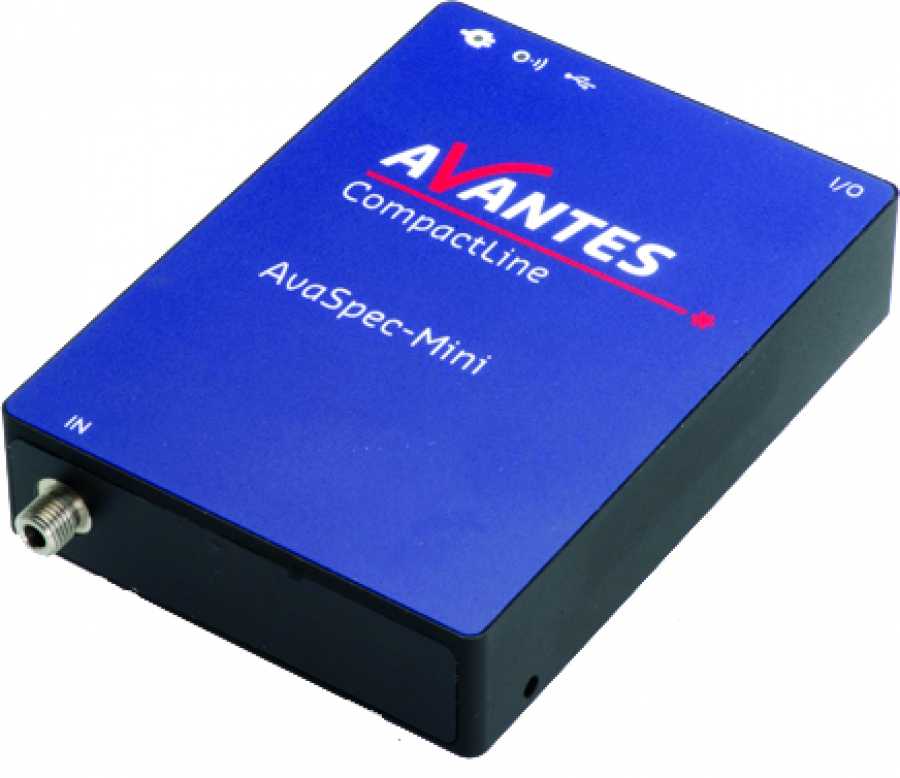
\includegraphics[width=.7\textwidth]{figures/avaspec-mini.png}
    }
  \end{minipage}
  \begin{minipage}{.49\textwidth}
    \subfloat[]{
      \centering setup sketch here
    }
  \end{minipage}
\caption[]{\textbf{Spectrometer Module.}}
\end{figure}

\newpage
\subsection{Liquid Flux: Continuous Culture \& Turbidostat} 
\label{cult}

\paragraph{Project:} build a module consisting of media and waste bottles, 
a reactor vessel, peristaltic pump(s), and a scale; pump and scale are
controlled \textit{via} serial interfaces from an
Arduino+Touchscreen. The flow rate is controlled \textit{via} the pump
motor speed and recorded \textit{via} the scale; the flow rate is
recorded or can be set after a setup-specific (tubing) calibration
routine


\begin{enumerate}
\item \build{} a simple reactor vessel (Schott bottles) with liquid
  media flow, from media bottles through reactor vessel and out to
  waste bottle 
\item \code{}: calibration routine for the weight sensor module
\item \code{}: analog control of peristaltic motor speed and recording of
  weight loss and/or gain to record mass flow (g/min)
\item \code{}: routine to calibrate pump speed to weight loss/gain
  for a specific setup; store calibration on SD card, which allows
  to also set pump speed in g/min, or if provided with a culture
  volume, as culture dilution rate (\ph{})
\item \build{} \& \code{}: combine with \ref{spec} to make
  turbidostatic control
\item \build{}: add gassing system of project \ref{gas} to make a first
  simple bioreactor
\end{enumerate}

\paragraph{Resources:}
\begin{itemize}
\item Arduino tutorials for
  \href{http://www.instructables.com/id/Control-peristaltic-pump-with-TA7291P-and-an-Ardui/}{Adafruit
    peristaltic pump} and general
  \href{http://playground.arduino.cc/TA7291PDCMOTORCONTROLLER/TA7291PDCMOTORCONTROLLER}{DC motor control} and \href{https://www.adafruit.com/products/1438}{Adafruit motor shield}
\item \href{http://www.elecrow.com/wiki/index.php?title=Weight_Sensor_Scales_Kit-_20KG}{Arduino library for Elecrow weight sensor kit 3 kg}
\item \href{https://cdn.sparkfun.com/datasheets/Sensors/ForceFlex/hx711_english.pdf}{HX711 24-bit analog-to-digital converter (ADC) for load cells}
\end{itemize}

\paragraph{Materials:}
\begin{itemize}
\item Bottles, screw caps with inlet/outlet openings,
  and tubing: \avail{} \& \obtain{}!
\item Scale - \ordered{}\\
  fancy:
  \href{http://de.mt.com/de/de/home/products/Industrial_Weighing_Solutions/bench-scales/weighing-platforms/high-resolution/PBK785.html}{Mettler Toledo, PBK785-3XS/f}\\cheap:
  \href{http://www.elecrow.com/weight-sensor-kit-3kg-p-883.html}{Elecrow
    Weight Sensor kit 3kg for Arduino} $\leftarrow$ \ordered{}
\item Peristaltic pumps - \ordered{}\\ fancy:
  \href{http://www.drifton.dk/de/product/lp-bt100-2j-13/}{Longer Pump
    LP-BT100-2J, DG-2(10)}\\cheap:
  \href{http://www.ismatec.com/int_e/pumps/t_ecoline/ecomsca4.htm}{Ismatec
    Ecoline VC-MS/CA4-12}\\ cheaper: \href{Welco WPM}{Welco WPM} or
  cheapest: \href{https://www.adafruit.com/product/1150}{Adafruit}
  $\leftarrow$ \ordered{}
\item Toshiba TA7291P Bridge Driver - \ordered{}
\item Sainsmart Arduino Mega + Touchscreen - \ordered{}
\end{itemize}

\begin{figure}[ht]
  \begin{minipage}{.49\textwidth}
    \subfloat[Elecrow Scale Module, 3 kg]{
      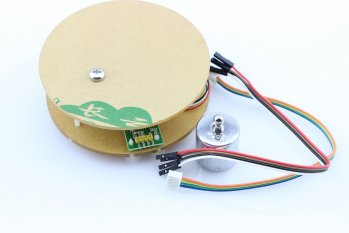
\includegraphics[width=.8\textwidth]{figures/elecrow_scale.png}
    }\\
    \subfloat[Adafruit Peristaltic Pump]{
      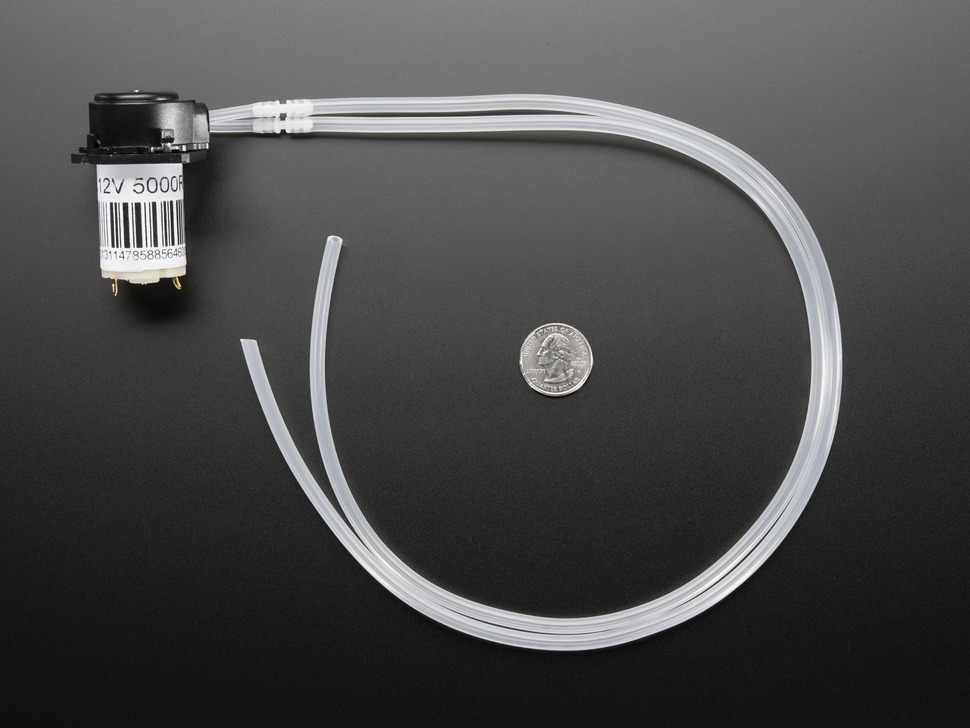
\includegraphics[width=.8\textwidth]{figures/adafruit_pump.png}
    }
  \end{minipage}
  \begin{minipage}{.5\textwidth}
    \subfloat[Fritzing scheme for the Pump]{
      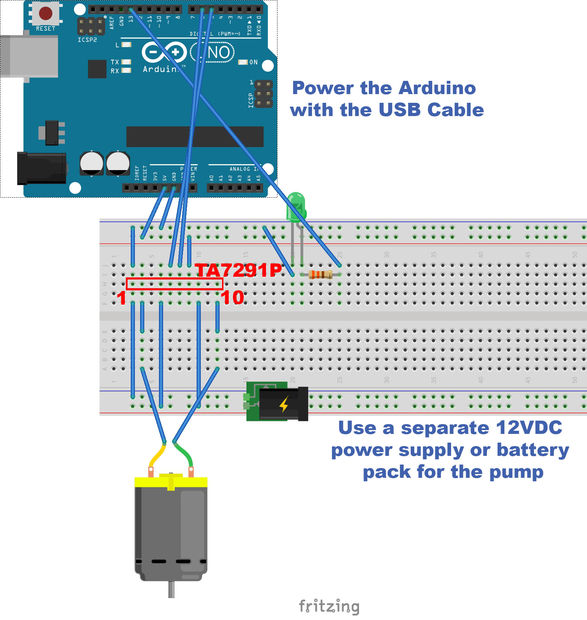
\includegraphics[width=\textwidth]{figures/pump_fritzing.png}
    }
  \end{minipage}
\caption[]{\textbf{Continuous Culture Module}. The elecrow scale
  module is based on the HX711 load-cell amplifier (24-bit analog-
  to-digital converter) and connected to 5V, Gnd and two analog pins
  of the Arduino and comes with an
  \href{http://www.elecrow.com/wiki/index.php?title=Weight_Sensor_Scales_Kit-_20KG}{Arduino
    library}. An \href{https://www.adafruit.com/product/1150}{Adafruit
    peristaltic pump} (12 v) is run by a ``geared down DC motor'' and
  requires a Toshiba TA7291P Bridge Driver (0-20V 1A; 2A peak) to
  control pump direction and speed \textit{via} Arduino's PWM pins,
  see the
  \href{http://www.instructables.com/id/Control-peristaltic-pump-with-TA7291P-and-an-Ardui/}{\textit{instructable}
    tutorial}.}
\end{figure}

\clearpage
\subsection{The Server}
\paragraph{Project:} a master software running on a (detachable) linux 
desktop that synchronizes and speaks via a comon interface to all
Arduino and Raspberry Pi modules; the modules themselves can interpret
get, set and act impulses (use arguments only when absolutely
necessary).\\ During an initializiation the server may inquire what an
attached module provides (\textit{via} data IDs and SI units,
meaningful time resolution) and handle it automatically. \\ Variable
higher order control or processing logics can be built using defined
data and control IDs. Ultimately, a direct integration with
mathematical models may be desirable.  For example, measured \ox{} and
\cox{} levels may be used to estimate metabolic activities, such as
catabolic ATP/ADP turnover; required data and equations can be loaded
and interpreted \textit{via} SBML encoded models.
\begin{enumerate}
\item \build{} combine of gas (\ref{gas}), liquid (\ref{cult})
  and light (\ref{spec}) modules into a bioreactor
\item \code{}: master program to synchronize and record data from
  the three modules
\item \code{}: combine e.g. \ref{spec} \& \ref{cult} to implement
  turbidostat control
\item \code{}: higher order data evaluation logics, \textit{eg.}, estimate
  metabolic rates from gas exchange measurements
\end{enumerate}


\paragraph{Materials:}
\begin{itemize}
\item \texttt{setTime(time\_t $t$)}: sets the current master time to
  all modules
\item \texttt{get(..., time\_t $t$)}: get all values, currently
  available (with a time stamp), or from a previous time $t$
%\item \texttt{set(..., time\_t $t$)}: sets specific values, now or at an
%  indicated future time $t$
\item \texttt{act(..., time\_t $t$)}: act (switch on and off, set to a
  specific value), now or at future time $t$
\end{itemize}

\newpage
\subsection{Heat Flux: Water Bath Thermostat}
\label{heat}

\paragraph{Project:} build a water bath for growth vessels, control
T, read-out energy required for maintaining constant T and estimate
the amount of heat withdrawn or administered

\begin{enumerate}
\item
\end{enumerate}

\paragraph{Materials:}
\begin{itemize}
\item Jacketed reactor vessel: \build{} or \obtain{}
\item Julabo water bath,
e.g. \href{http://www.laborhandel24.de/9162625-de?utm_source=google_shopping&gclid=Cj0KEQiA496zBRDoi5OY3p2xmaUBEiQArLNnK6uWkryhjvkNdmRLgcg2W_HIO9W1aKaKCO9gmvlkt_MaAmhe8P8HAQ}{F25-ME}
\item Arduino and/or Raspberry Pi
\end{itemize}

\newpage
\subsection{The \texttt{Kaiten Eppi}: Automated Sampling Device} 
\label{sampling}
\paragraph{Projects:} build sterile and automated sampling device; using
a controllable syringe pump, sampling into the \texttt{Kaiten Eppi}
(automated: pump sample into tubes, potentially pre-filled with
chemicals, vortex, and transport them into liquid N$_2$ or other
storage containers)

\paragraph{Materials:}
\begin{itemize}
\item Sterile sampling device by HHU glas blowers: \avail{}
\item Syringe pump: \obtain{}
\item \texttt{Kaiten Eppi}: \build{}
\item Sainsmart Arduino Mega \& Touchscreen: \obtain{}
\end{itemize}


\newpage
\subsection{Single Cell Biology: Microfluidic Device} 
\label{micro}

\paragraph{Project:} Basic microfluidics and live-cell imaging device;
scratch growth chambers and liquid flow channels into microscope slide;
attach 2--3 pumps; and control \textit{via} arduino/screen

\paragraph{Resources:}
\begin{itemize}
\item \href{http://www.ncbi.nlm.nih.gov/pmc/articles/PMC4641590/}{Tsuda \textit{et al.} PLoS ONE 2015: 3D Printed 'Plug and Play' Millifluidic}
\end{itemize}

\paragraph{Materials:}
\begin{itemize}
\item Ilka's lab microscope: \avail{}
\item Microscopy slides: \avail{}
\item 2--3 peristaltic pumps for microfluidics: \obtain{}
\item Sainsmart's Arduino Mega + Touchscreen: \obtain{}
\end{itemize}


\newpage

\subsection{Participants \& Teams}

\begin{table}[ht!]
  \begin{tabular}{lllc}
    \bf type & \bf name & \bf e-mail & \bf team \\\hline
    & Sascha Wigger & sascha.wigger@student.htw-berlin.de&\\
    & Nicolas Schmelling & nicolas.schmelling@uni-duesseldorf.de&\\
    & Fiona Moejes & fionamoejes@hotmail.com &\\
    & Stefano Magni & stefano.magni@uni-duesseldorf.de&\\
    & Philipp Norf & philipp.norf@uni-duesseldorf.de&\\
    & Elahe Radmaneshfar & radmaneshfar@gmail.com&\\
    & Anna Matuszynska & anna.matuszynska@hhu.de&\\
    & Suraj Sharma & suraj.sharma@uni-duesseldorf.de&\\
    & Simon Schliesky & simon.schliesky@hhu.de&\\
    & Antonella Succurro & succurro@hhu.de& \\
    & Robert Lehmann & lehmann.rob@googlemail.com &\\
    & Dougie Murray & dougie@ttck.keio.ac.jp&\\
    & Oliver Ebenh\"oh & oliver.ebenhoeh@hhu.de& \\
    & Rainer Machn\'e & machne@hhu.de& 
  \end{tabular}
  \caption[]{should we have skill badges, \url{https://www.adafruit.com/products/2857?q=skill\%20badge&p=0&} or 3D-printed awards, like the ``red soldering iron'', ``the blue tube'', ``the green chip''?}
\end{table}

\section{Outlook: 2$^{nd}$ QTB PBR \hack{}}

\subsection{\textit{Growth Dynamics}: Photobioreactors in Research}

Talks, 30-60 min:

Nir Keren, Hellingwerf, Jan Cerveny, Dougie Murray,
something microfluidics?

\subsection{\textit{Single Cell Dynamics}: Microfluidic Devices}
Integrate project \ref{micro} with the simple microscope in
Ilka's lab, or a more advanced system (CAi?)

%\subsection{Growth Dynamics}

\subsection{\textit{Omics}: Sterile and Automated Sampling Devices}

Proper sampling for high-throughput data acquisition (mass
spectrometry, sequencing) - the \texttt{Kaiten Eppi}

\end{document}
